\chapter{Graph Tracking in Probabilistic Models}
\label{cha:graph-track-prob}

The system described in chapter~\ref{cha:impl-dynam-graph}, implemented in a Julia package
\irtrackerjl{}, can now be utilized for the analysis of probabilistic models written in \dppljl{},
and for posterior inference in \turingjl{}.  This part of the work is realized in another package,
\autogibbsjl{}, which is available as open-source
code\footnote{\url{https://github.com/phipsgabler/AutoGibbs.jl}}.  There are two applications
provided, built on top of the graph tracking functionality: first, dependency analysis of random
variables in a model can be performed.  This results in the complete graphical model for static
models, and a slice of it for dynamic models.  The resulting graph can be plotted for visualization.
Second, given the dependency graph, the conditional likelihoods of unobserved variables in static
models can be extracted.  With these, analytic Gibbs conditionals can be derived and used in
\turingjl{}'s within-Gibbs sampler.

\section{Dependency Analysis in Dynamic Models}
\label{sec:depend-analysis}

Context for DPPL-models; slicing; graph extraction + new representation; plotting

\begin{lstfloat}[t]
\begin{lstlisting}[style=lstfloat]
@model function bernoulli_mixture(x)
    w ~ Dirichlet(2, 1/2)
    p ~ DiscreteNonParametric([0.3, 0.7], w)
    x ~ Bernoulli(p)
end

@model function hierarchical_gaussian(x)
    λ ~ Gamma(2.0, inv(3.0))
    m ~ Normal(0, sqrt(1 / λ))
    x ~ Normal(m, sqrt(1 / λ))
end
\end{lstlisting}
  \caption{Two simple example models: a mixture of two Bernoulli random variables with fixed
    probabilities, and a Gaussian model with conjugate prior.  Both models are defined over one
    single observation.}
  \label{lst:dependency-examples}
\end{lstfloat}

\begin{figure}[t]
  \centering
  \subbottom[][\protect\jlinl{bernoulli_mixture}]{%
    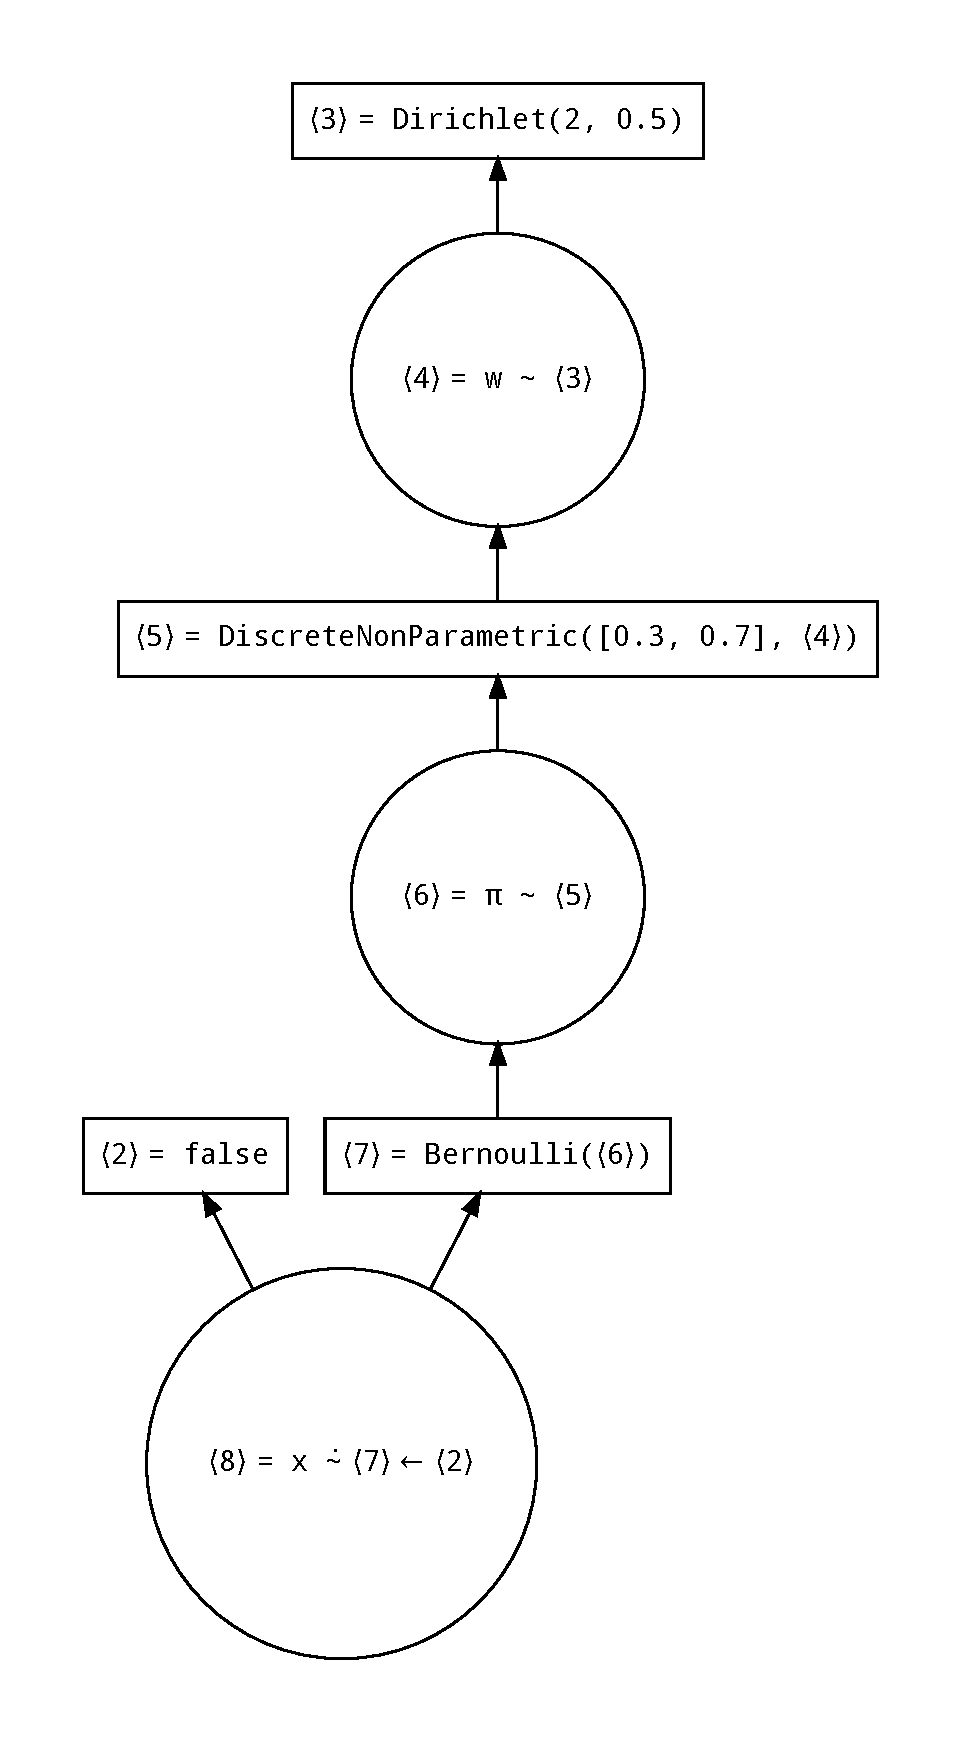
\includegraphics[width=0.48\textwidth]{figures/bernoulli_dependencies}}
  \subbottom[][\protect\jlinl{hierarchical_gaussian}]{%
    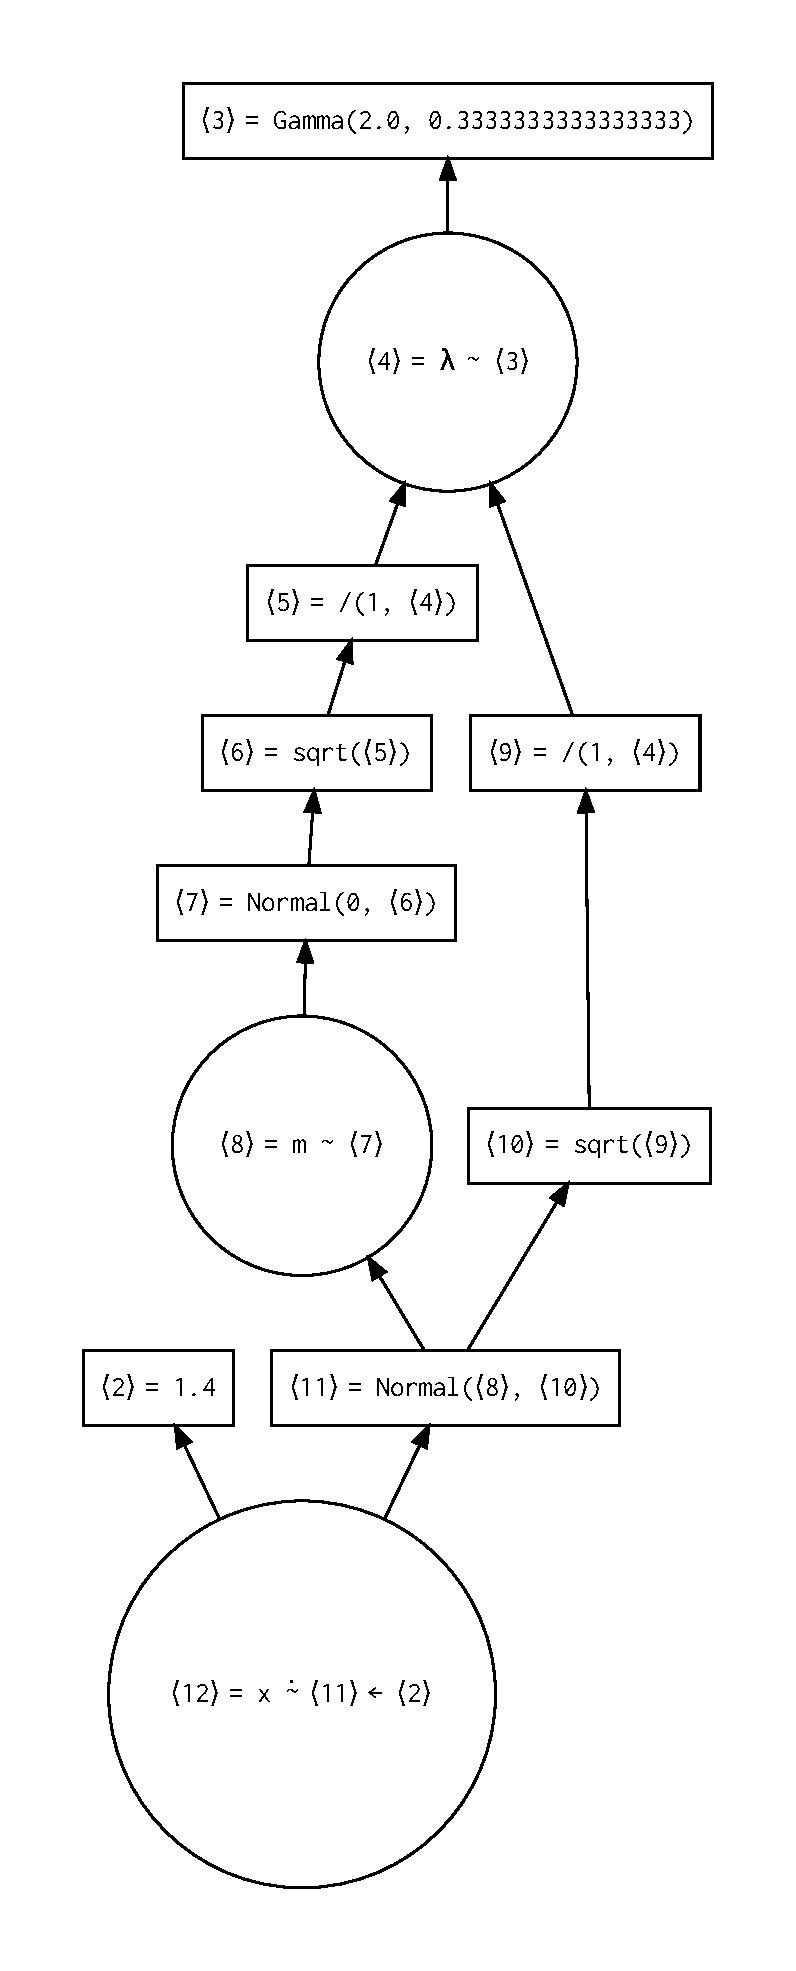
\includegraphics[width=0.48\textwidth]{figures/gaussian_dependencies}}
  \caption{Dependency graphs of the models in \ref{lst:dependency-examples}.  More information (such
    as variable names and values of nodes) is stored in the real model graph, but not shown for ease
    of visualization.}
  \label{fig:geom-deps}
\end{figure}

% ⟨2⟩ = false
% ⟨3⟩ = Dirichlet(2, 0.5) → Dirichlet{Float64}(alpha=[0.5, 0.5])
% ⟨4⟩ = w ~ ⟨3⟩ → [0.826304431175434, 0.17369556882456608]
% ⟨5⟩ = DiscreteNonParametric([0.3, 0.7], ⟨4⟩) → DiscreteNonParametric{Float64,Float64,Array{Float64,1},Array{Float64,1}}(support=[0.3, 0.7], p=[0.826304431175434, 0.17369556882456608])
% ⟨6⟩ = p ~ ⟨5⟩ → 0.3
% ⟨7⟩ = Bernoulli(⟨6⟩) → Bernoulli{Float64}(p=0.3)
% ⟨8⟩ = x ⩪ ⟨7⟩ ← ⟨2⟩

% julia> graph0 = trackdependencies(hierarchical_gaussian(1.4))
% ⟨2⟩ = 1.4
% ⟨3⟩ = Gamma(2.0, 0.3333333333333333) → Gamma{Float64}(α=2.0, θ=0.3333333333333333)
% ⟨4⟩ = λ ~ ⟨3⟩ → 0.9257859525673857
% ⟨5⟩ = /(1, ⟨4⟩) → 1.0801632896100921
% ⟨6⟩ = sqrt(⟨5⟩) → 1.0393090443222806
% ⟨7⟩ = Normal(0, ⟨6⟩) → Normal{Float64}(μ=0.0, σ=1.0393090443222806)
% ⟨8⟩ = m ~ ⟨7⟩ → 1.8505166567138398
% ⟨9⟩ = /(1, ⟨4⟩) → 1.0801632896100921
% ⟨10⟩ = sqrt(⟨9⟩) → 1.0393090443222806
% ⟨11⟩ = Normal(⟨8⟩, ⟨10⟩) → Normal{Float64}(μ=1.8505166567138398, σ=1.0393090443222806)
% ⟨12⟩ = x ⩪ ⟨11⟩ ← ⟨2⟩



\section{JAGS-Style Automatic Calculation of Gibbs Conditionals}
\label{sec:jags-style-conditionals}

Gibbs sampler implementation for Turing; likelihood closures; conditional likelihood extraction


\section{Evaluation}
\label{sec:autogibbs-eval}

\begin{table}[t]
  \centering
  \libertineTabular
  \begin{tabular}{llrrrrrrr}
    \toprule
    Algorithms & & \multicolumn{3}{c}{GMM} & \multicolumn{3}{c}{HMM} & \multicolumn{1}{c}{IMM} \\
    \midrule
    AG + HMC & Data size & 10 & 25 & 50 & 10 & 25 & 50 & 10 \\
    & Chains & 30 & 30 & 30 & 30 & 30 & 30 & 30 \\
    & Compilations & 3 & 3 & 3 & 3 & 3 & 3 & 3\\
    \addlinespace
    PG + HMC, & Data size & 10 & 25 & 50 & 10 & 25 & 50 & 10 \\
    10 particles & Chains & 10 & 10 & 10 & 10 & 10 & 10 & 10 \\
    \addlinespace
    PG + HMC, & Data size & 10 & 25 & 50 & 10 & 25 & 50 & 10 \\
    25 particles & Chains & 10 & 10 & 10 & 10 & 10 & 10 & 10 \\
    \addlinespace
    PG + HMC, & Data size & 10 & 25 & 50 & 10 & 25 & 50 & 10 \\
    50 particles & Chains & 10 & 10 & 10 & 10 & 10 & *x & 10 \\
    \bottomrule
  \end{tabular}
  \caption{Experimental combinations that were run.  Chains were always of length \(5000\).  The
    parameters for HMC were a stepsize of \(0.1\), and \(10\) leapfrog steps.  A new static Gibbs
    conditional was extracted for each block of \(10\) chains that was run with the same parameters
    while Particle Gibbs was varied over the three particle sizes.  Particle Gibbs with 50 particles
    was sometimes killed due to timeouts on the server.}
  \label{tab:autogibbs-params}
\end{table}

\begin{equation}
  \label{eq:gmm}
  \begin{aligned}
    \mu_{k} &\from \Normal(0, \sigma_{1}), \quad k = 1, \ldots, K \\
    w &\from \distr{Dirichlet(K)} \\
    z_{n} &\from \distr{Discrete}([1, \ldots, K], w), \quad n = 1, \ldots, N \\
    x_{n} &\from \Normal(\mu_{z_{n}}, \sigma_{1}), \quad n = 1, \ldots, N
  \end{aligned}
\end{equation}

\begin{equation}
  \label{eq:hmm}
  \begin{aligned}
    T_{k} &\from \distr{Dirichlet}(K), \quad k = 1, \ldots, K \\
    m_{k} &\from \Normal(k, \sigma_{1}), \quad k = 1, \ldots, K \\
    s_{1} &\from \distr{Categorical}(K) \\
    s_{k} &\from \distr{Categorical}(T_{s_{k-1}}), \quad k = 2, \ldots, N \\
    x_{k} &\from \Normal(m_{s_{k}}, \sigma_{2}), \quad k = 1, \ldots, N
  \end{aligned}
\end{equation}

\begin{equation}
  \label{eq:imm}
  \begin{aligned}
    w &\from \distr{TruncatedStickBreakingProcess(\alpha, K)} \\
    z_{n} &\from \distr{Categorical}(w), \quad n = 1, \ldots, N \\
    \mu_{k} &\from \Normal(0, \sigma_{1}), \quad k = 1, \ldots, K \\
    y_{n} &\from \Normal(\mu_{z_{n}}, \sigma_{2}), \quad n = 1, \ldots, N
  \end{aligned}
\end{equation}

% extraction times
% Measuring both compilation of the traced code and the conditional calculation.",
% "All 2 or 3 repetitions per data size class are shown."
% Linear fit for time ~ datasize²
% three samples

% sampling times
% subtitle = "Factored by algorithm and number of PG particles"

% diagnostics
% subtitle = "Factored by algorithm and number of particles"

% densities
% subtitle = paste("Factored by number of observations (data size)", "and selected parameters")

% ACFs
% subtitle = "ACF plots for one sample chain per data size"


%%% Local Variables: 
%%% TeX-master: "main"
%%% End: